\documentclass[12pt,letterpaper]{hmcpset}
\usepackage[margin=1in]{geometry} 
\usepackage{graphicx}
\usepackage{amsmath}
\usepackage{boxedminipage}
\usepackage{url}
\usepackage{geometry}

% info for header block in upper right hand corner
\name{}
\class{Math 45 - Section --- \hspace{20pt}}
\assignment{HW 10}
\duedate{Friday, April 22, 2016}

\newcommand{\pn}[1]{\left( #1 \right)}
\newcommand{\abs}[1]{\left| #1 \right|}
\newcommand{\bk}[1]{\left[ #1 \right]}

% Start enumerates at a) instead of 1
\renewcommand{\labelenumi}{{(\alph{enumi})}}

%Block Paragraphs
\setlength{\parindent}{0pt}
\setlength{\parskip}{1em}

\begin{document}

\problemlist{1, 2, 3}

\begin{problem}[1]
    On the midterm, you were asked to solve the nonlinear differential equation $y'(t)=4t\sqrt{y}$ with the initial condition $y(1)=y_0$.  If $y_0=0$, this IVP does not have a unique solution (since $y(t)=0$ is a second solution). If $y_0\neq 0$, this IVP has a unique solution. And yet, Wolfram Alpha and Mathematica both give two solutions to the IVP with $y(1)=9$.

    \begin{center}
        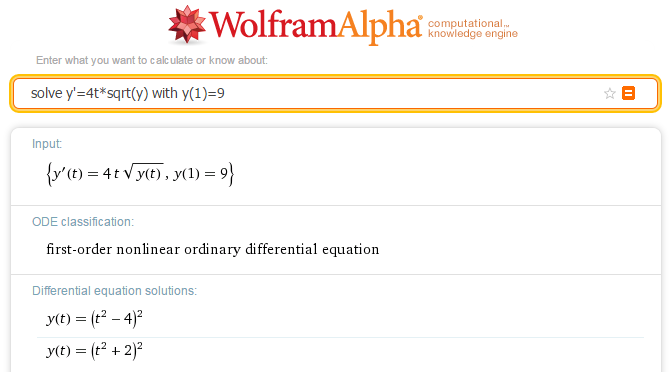
\includegraphics[width=6in,keepaspectratio=true]{img/apr_22_1_wolfram_.png}
    \end{center}

    \begin{enumerate}
        \item First, solve the IVP with $y(1)=9$. Try to understand why Wolfram Alpha comes up with both solutions.
        \item Only one of the two solutions is the correct solution to the IVP.  Determine which one is correct and why.
    \end{enumerate}
    \textbf{Note:} This problem is a great example of why computers and calculators are mathematical aids, but they don't replace mathematically proficient humans who can think carefully. \textit{If you use a computer or calculator to do mathematics, always check if the answer is correct or at least reasonable.}
\end{problem}

\newpage
%p1%
\begin{solution}
    \null\vfill
\end{solution}
\newpage

%p2%
\begin{problem}[2]
    Here are five physical scenarios that involve oscillations.  In each, identify the source of damping (if it is present) that causes oscillations to die out over time, and any relevant forcing (inputs) to the system that might cause it to oscillate.
    \begin{enumerate}
        \item Tall buildings can sway (with period of motion on the order of a few seconds)
        \item Water sloshing around in a cup
        \item Violins, pianos, any stringed instrument
        \item Shock absorbers in a car
        \item (Make up your own)
    \end{enumerate}
\end{problem}

\begin{solution}
    \vfill
\end{solution}
\newpage

%p3%
\begin{problem}[3]
    Examine Student P's work on the following problem.  What did the student do correctly?  What mistake(s) did the student make?  What is a more correct response to the problem, and what would you say to help the student understand how to correctly complete the problem?

    \begin{center}
        \framebox{\parbox[c]{5.5in}{Solve the IVP $y''+4y=t^2$ subject to $y(0)=0$ and $y'(0)=1$.

        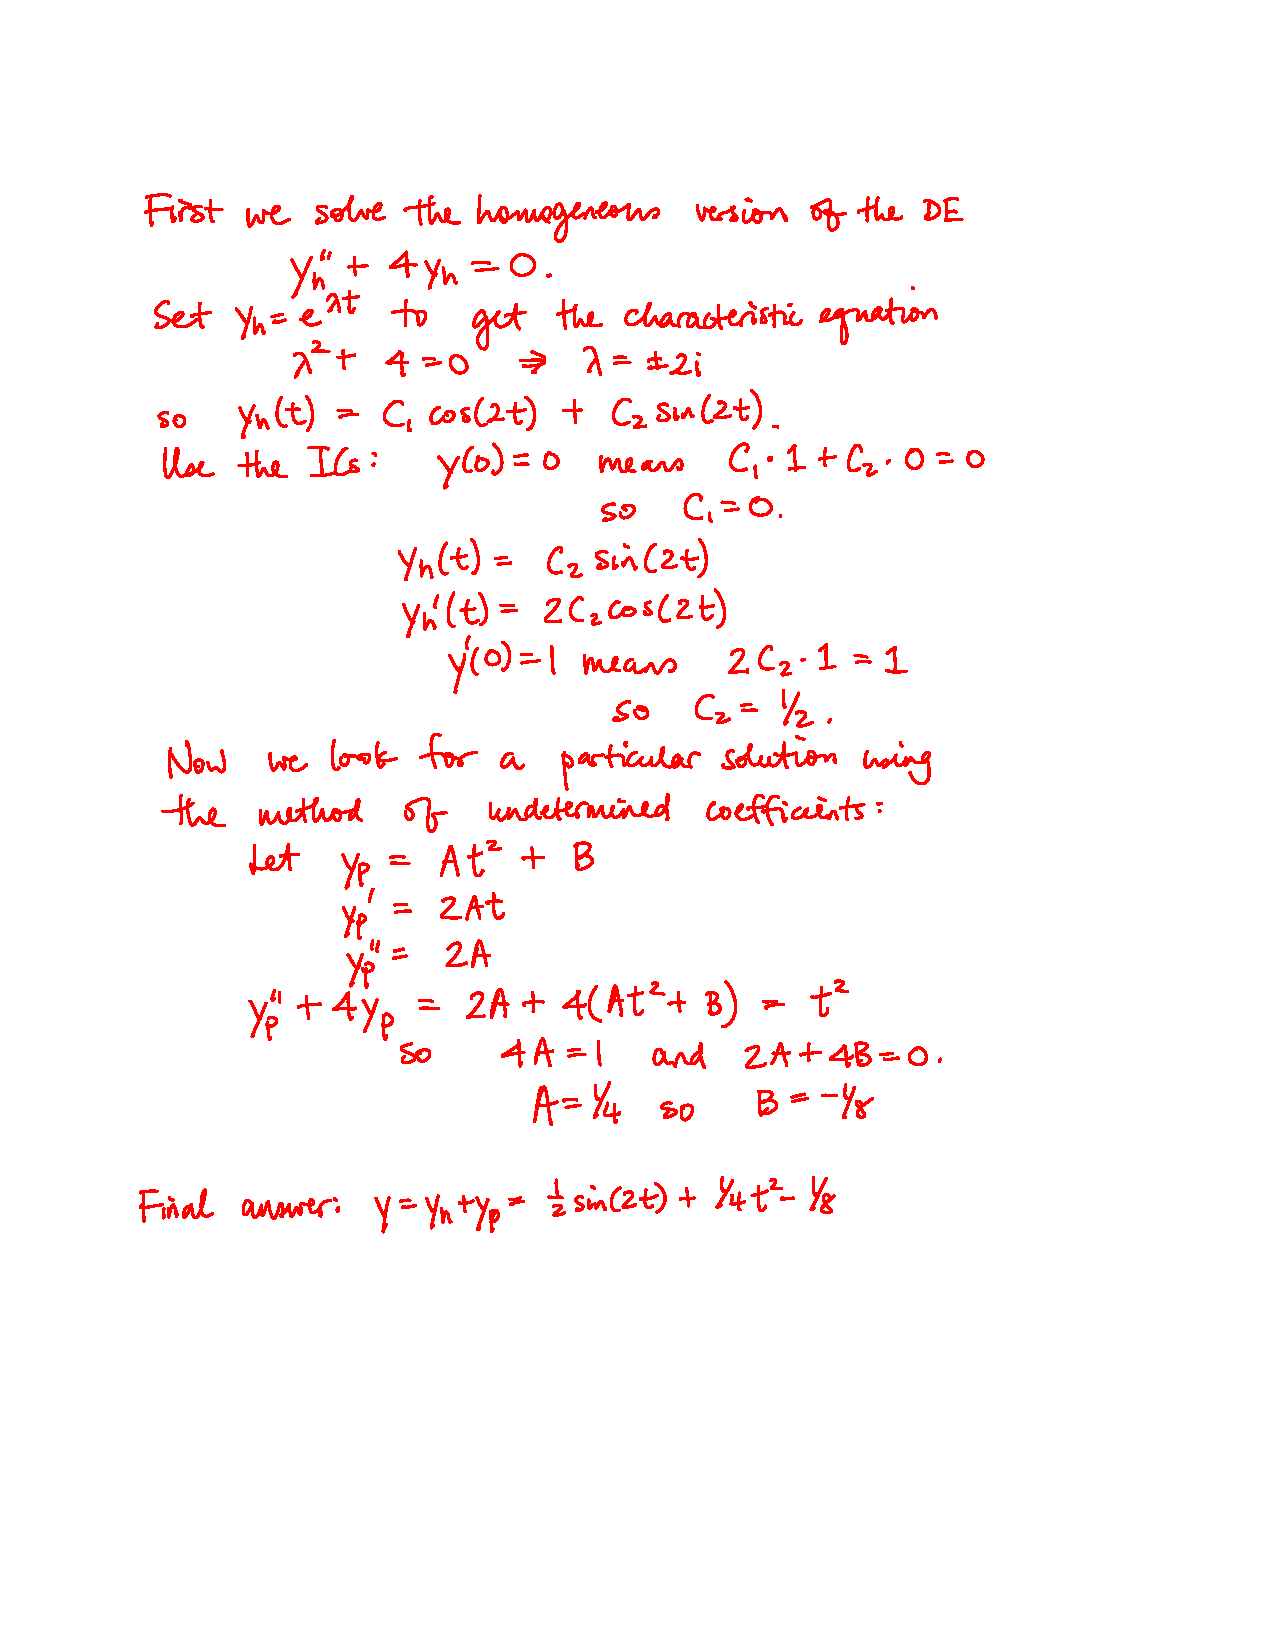
\includegraphics[width=4in,keepaspectratio=true]{img/apr_22_5_misonception.pdf}}}
    \end{center}
\end{problem}

\newpage
\begin{solution}
    \null\vfill
\end{solution}
\newpage

%p4%
\begin{problem}
    \textbf{Instructions on final project:} 
    \begin{itemize}
        \item Please continue to work on your Math 45 final project.  We suggest each of you put in at least three hours of work into your final project this week. 
        \item Strive to have each person contribute a fair and equitable amount of work and decision-making into the project. 
        \item Start thinking ahead about how you want to communicate your findings to the rest of the class.  Each group is limited to 4.5 minutes.  (We are allowing time for questions on top of that.)  Each person should have a role during the presentation.  If you want to create a set of presentation slides, look on our Sakai site for a PowerPoint template.  
    \end{itemize}
\end{problem}
\end{document}
